\newpage
\section{Signal Converter}
The primary purpose of this block is to convert the output from the Torque Sensor to a signal which can be correctly measured by the Control Unit.

\subsection{Design}
The torque-signal and the velocity-signal from the Torque Sensor are measured by the PSoC using different techniques and the Signal Converter must therefore be in charge of three different signal-processing techniques: Rescaling the torque-signal and reduce the noise in the velocity-signal.

\textbf{Rescaling torque-signal}\\
As the PSoC can only measure voltage-levels ranging from $0$ to $+5 V$, and the output-signal from the torque measurement lies between $-5 V$ to $+5 V$, it is necessary to rescale the signal such that the PSoC's input-signal can be described using this formula:
\begin{equation}
	V_t = \frac{\tau_{sensor} }{2} + 2.5 V
\end{equation}

The desired signal can be found by amplifying the input-signal with a factor 0.5 and then lifting the signal with an offset of $\SI{2.5}{\volt}$. This can be done using a non-inverting adder.

\begin{figure}[H]
	\centering
	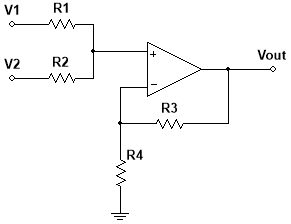
\includegraphics[width=0.4\linewidth]{Hardware/SignalConverter/TorqueDesign1}
	\caption{Non-inverting adder using operational amplifier}
	\label{fig:SignalConverterTorque1}
\end{figure}

A non-inverting adder is similiar to a non-inverting amplifier but contains a voltage divider on the Op-amps non-inverting input. The design is based on equally sized resistors:
\begin{equation}
	R_1 = R_2 = R_3 = R_4
\end{equation}
Due to the high-impedance of the op-amp, no current flows into the input. he current I\textsubscript{P} can be therefore bee calculated using Ohm's law:
\begin{equation}
	I_P = \frac{V_1 - V_2}{R_1 + R_2} = \frac{V_1 - V_2}{2 \cdot R}
\end{equation}
The voltage on the op-amps non-inverting input can be calculated as:
\begin{equation}
	V_P = V_1 - V_2 = V_1 - I_P \cdot R = V_1 - \frac{V_1 - V_2}{2 \cdot R} \cdot R = \frac{V_1 + V_2}{2}
\end{equation}
\newpage
Due to the operational amplifier's feedback-connection it will function as a non-inverting amplifier. This amplification can be found as:
\begin{equation}
	A = 1 + \frac{R}{R} = 2
\end{equation}
This means that the op-amps output-voltage can be calculated as:
\begin{equation}
	V_{out} = V_P \cdot A = \frac{V_1 + V_2}{2} \cdot 2 = V_1 + V_2
\end{equation}
The signals V\textsubscript{1} is the $\pm \SI{5}{\volt}$ signal from the Torque Sensor. The signal's voltage is cut in half using a voltage divider. The signal V\textsubscript{2} is the 5 VDC supply which can be used to add a $\SI{2.5}{\volt}$ offset to the input. This is also done using a voltage divider. Both voltage dividers can be made using only $\SI{10}{\kilo \ohm}$ resistors. This resistor-value is also used in the rest of the design. This leads to the final design seen below:

\begin{figure}[H]
	\centering
	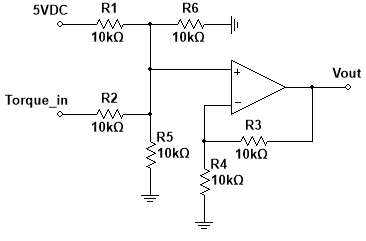
\includegraphics[width=0.5\linewidth]{Hardware/SignalConverter/TorqueDesign2}
	\caption{Circuit diagram for Signal Converter (torque-signal)}
	\label{fig:SignalConverterTorque2}
\end{figure}
\textbf{Noise reduction in velocity-signal}\\
The output-signal for the measured angular velocity lies between the $0$ to $+5 V$ range and can therefore be measured correctly by the PSoC without rescaling. However, the electrical noise in the signal must be reduced, in order to let the PSoC measure correctly.

The noise can be reduced with a low-pass filter, but if it is assumed that the amplitude of the noise is low enough it can also be reduced using a comparator with hysteresis. This comparator must be fast enough to convert the signal and the highest frequency of the velocity-signal must be calculated.

From the analysis of the Generator it was found that the rolls angular velocity $\omega_{Roll}$ is equal to 1047 rpm - when AU2 runs at cruise speed (maximum velocity). This velocity will create a velocity-signal with the highest frequency. This frequency can be found as:
\begin{equation}
	f_{v} = 360 \frac{pulses}{rotation} \cdot \frac{\omega_{Roll}}{60\frac{seconds}{minutes}} = \SI{6.282}{\kilo \hertz}
\end{equation}

\subsection{Implementation}
The designs from the previous section is implemented using a non-inverting adder and two schmitt-triggers in series.

\textbf{Non-inverting adder}\\
The circuit is built using a MCP601 operational amplifier. Its positive and negative supply lines are connected with 5 VDC and ground. The op-amps positive power supply is parallel-connected with a capacitor. This capacitor improves the op-amps high-frequency response.

\textbf{Schmitt-trigger}\\
The noise reduction is implemented using two 74HC14 hex inverter with Schmitt-trigger inputs. The inverter creates a small propagation delay between the Torque Sensor's output and the PSoC's input. At a 5VDC power supply this delay is given by:
\begin{equation}
	t_{pd} = t_{PHL} = t_{PLH} = \SI{24}{\nano \second}
\end{equation}

\begin{figure}[H]
	\centering
	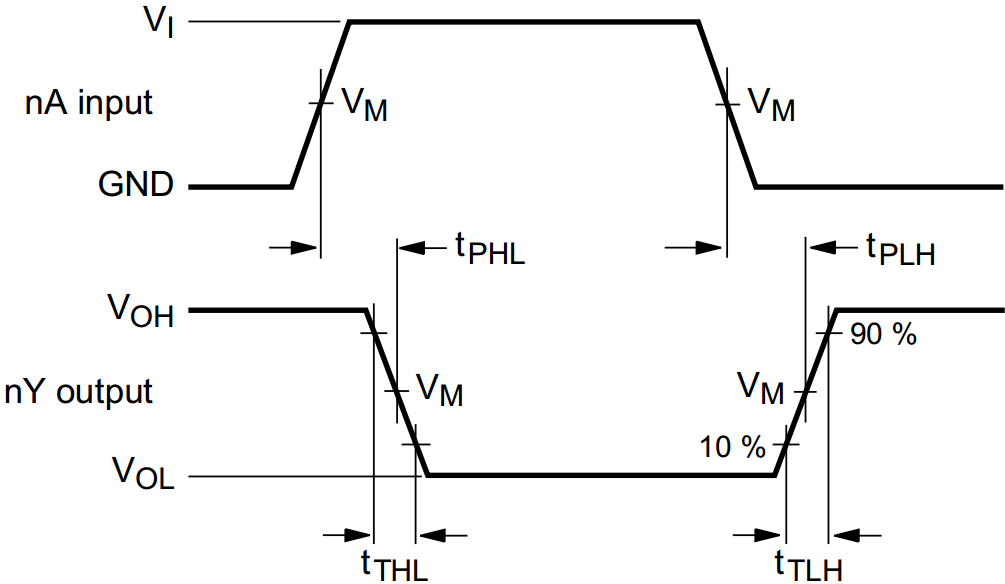
\includegraphics[width=0.5\linewidth]{Hardware/Pictures/74HC14_waveform}
	\caption{Typical inverter-waveform}
	\label{fig:SchmittTrigger_waveform}
\end{figure}

In order to counter the inverting property of 74HC14, and create a comperator, the noise reduction  must consist of two Schmitt-triggers in series. This gives the subsystem a total propagation delay of $\SI{24}{\nano \second}$. As the 74HC14 contains six Schmitt-triggers the 4 unused Schmitt-trigger's inputs are connected to ground in order to prevent unwanted oscilliation.

\subsection{Unity test}
Text